%%%%%%%%%%%%%%%%%%%%%%%%%%%%%%%%%%%%%%%%%%%%%%%%%%%%%%%%%%%%%%%%%%%%%%
% BAB TINJAUAN PUSTAKA
%=====================================================================
\renewcommand{\thechapter}{\Roman{chapter}}
\addtocontents{toc}{\vskip10pt}
\chapter{TINJAUAN PUSTAKA}
\renewcommand{\thechapter}{\arabic{chapter}}
%---------------------------------------------------------------------
\section{Stanene}
\begin{figure}
    \centering
    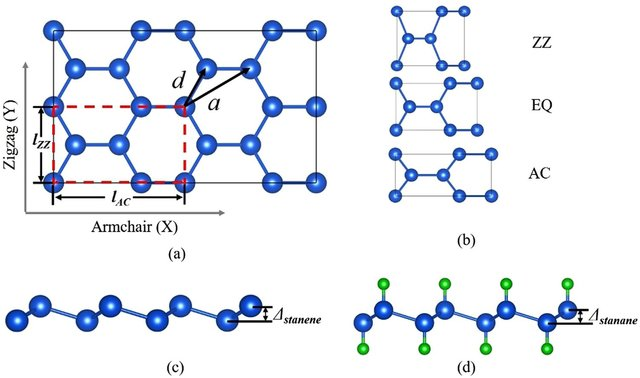
\includegraphics[width=17cm]{./gambar/struktur stanene.jpg}
    \caption{struktur dari material 2D stanene \citep{lu2017}}
    \label{struktur stanene}
\end{figure}
Stanene, bahan yang berasal dari timah (Sn) dalam bentuk lapisan dua dimensi dengan struktur yang mirip dengan graphene, telah menarik perhatian yang signifikan dalam beberapa tahun terakhir karena potensi aplikasinya dalam teknologi elektronik masa depan. Stanene pertama kali diusulkan oleh \citep{He2019} sebagai material topologis yang memiliki sifat konduktivitas elektronik yang luar biasa pada suhu kamar . Sifat ini berasal dari topologi elektroniknya yang memungkinkan pergerakan elektron tanpa hambatan di sepanjang tepinya, yang membuatnya sangat menarik untuk aplikasi dalam elektronik berenergi rendah .

Pada dasarnya, stanene adalah salah satu dari material topological insulator, di mana interior material berfungsi sebagai insulator sementara permukaannya mendukung arus listrik tanpa disipasi energi yang signifikan. Karakteristik unik ini disebabkan oleh adanya interaksi spin-orbit yang kuat pada atom timah, yang menyebabkan pembalikan pita energi dan pembentukan edge states yang terproteksi topologis . Penelitian eksperimental oleh \citep{zhu2015} menunjukkan bahwa stanene juga memiliki potensi sebagai bahan untuk transistor yang dapat beroperasi pada suhu kamar dengan efisiensi energi yang lebih tinggi dibandingkan dengan bahan konvensional seperti silikon.

Sifat-sifat unik stanene, seperti efek Hall kuantum spin (Quantum Spin Hall Effect), dihasilkan dari interaksi spin-orbit yang kuat pada atom timah. Ini menghasilkan pembalikan pita energi yang penting dalam pembentukan state topologi yang terlokalisasi di tepi material . Penelitian oleh \citep{PhysRevLett.111.136804} menunjukkan bahwa stanene, dengan struktur bandnya yang khas, dapat menghasilkan edge states yang dilindungi oleh simetri topologi, memungkinkan transportasi elektronik tanpa disipasi energi yang signifikan.

\citep{niuniu2022} melanjutkan dengan menggunakan DFT untuk mengeksplorasi bagaimana doping dengan elemen-elemen seperti bismut atau antimon dapat memodifikasi sifat elektronik stanene. Mereka menemukan bahwa doping dapat membuka celah pita energi yang lebih besar dan meningkatkan stabilitas struktural material, yang penting untuk aplikasi dalam perangkat elektronik canggih. Penelitian lebih lanjut oleh \citep{wu2020} menggunakan DFT untuk mengkaji dampak tegangan mekanik pada stanene. Hasilnya menunjukkan bahwa penerapan tegangan tertentu dapat memperluas atau mempersempit celah pita energi stanene, memungkinkan penyesuaian sifat elektronik material untuk berbagai aplikasi.

Penelitian eksperimental yang dilakukan oleh \citep{zhu2015} menunjukkan bahwa lapisan stanene dapat diproduksi secara epitaksial pada berbagai substrat, membuka jalan untuk integrasi dalam teknologi sirkuit terpadu dan perangkat spintronik . Pengembangan lebih lanjut dalam metode sintesis dan manipulasi stanene diharapkan akan membuka peluang baru untuk aplikasi dalam perangkat elektronik dengan efisiensi energi yang lebih tinggi dan kinerja yang lebih baik dibandingkan dengan material konvensional seperti silikon.

\begin{figure}
    \centering
    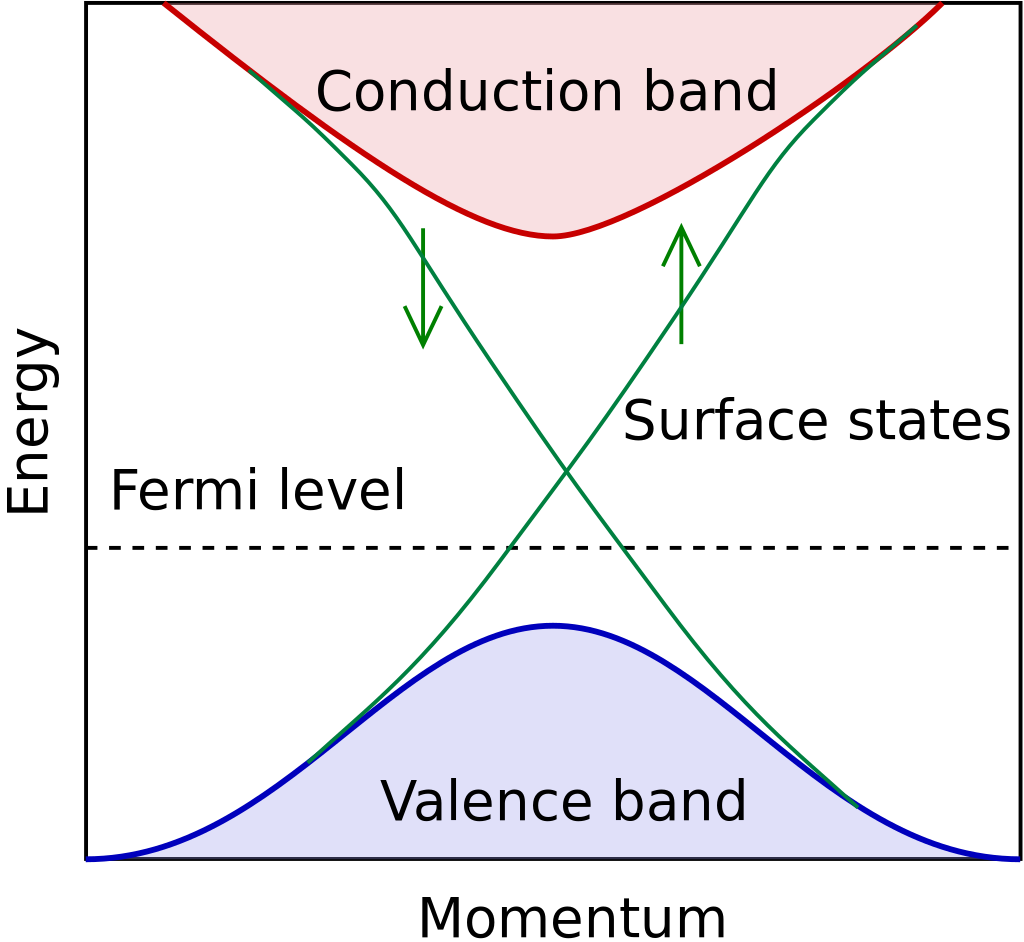
\includegraphics[width=10cm]{gambar/Topological_insulator_band_structure.png}
    \caption{Stuktur pita yang ideal untuk isolator topologi simetris pembalikan waktu 3D. Tingkat Fermi berada dalam celah pita bulk yang dilalui oleh kondisi permukaan Dirac bertekstur spin yang terlindungi secara topologis.}
    \label{band gap isolator topologis}
\end{figure}



%=====================================================================
\section{Teori Fungsional Densitas (\textit{Density Functional Theory})}
%=====================================================================
Salah satu kunci perkembangan sains dan teknologi adalah bagaimana kita bisa memahami dan mengatur sifat dari material dalam skala atom dan molekul secara individual. \textit{Density Functional Theory} (DFT) menjadi pendekatan yang sukses dalam penentuan solusi persamaan fundamental dalam fisika kuantum, yaitu persamaan \schro. DFT berkembang sangat pesat, dari sebuah teori yang digunakan sebagaian kecil oleh fisikawan menjadi dasar praktis bagi penelitian berbasis ilmu material, kimia, geologi, dll. Secara garis besar DFT merupakan teori tentang energi total, densitas elektron, dan relasinya dengan keadaan dasar (\textit{ground state}).

\subsection{Persamaan \schro}
Persamaan Schrödinger dikembangkan oleh fisikawan Austria bernama Erwin Schrödinger pada tahun 1925. Persamaan ini menyajikan fondasi teoretis yang kuat untuk memahami struktur elektron di atom dan memprediksi spektrum energi mereka. Persamaan ini berdasarkan pada konsep bahwa partikel subatom memiliki sifat gelombang dan partikel secara bersamaan. Dengan kata lain, persamaan Schrödinger menggambarkan partikel sebagai fungsi gelombang yang berubah seiring waktu. 
\begin{equation}
i\hbar \frac{\partial \Psi(\mathbf{r}, t)}{\partial t} = -\frac{\hbar^2}{2m} \nabla^2 \Psi(\mathbf{r}, t) + V(\mathbf{r})\Psi(\mathbf{r}, t)
\end{equation}

Namun, ketika kita mencoba mengaplikasikan persamaan Schrödinger pada sistem ril yang melibatkan banyak inti dan elektron, tantangan yang kompleks muncul. Salah satu masalah utamanya adalah ketidakmampuan untuk menyelesaikan persamaan tersebut secara analitik. Pada tahun 1929 \citeauthor{dirac1929quantum} mengatakan bahwa teori umum kuantum sudah hampir lengkap, namun kendalanya ialah mengaplikasikan teori-teori tersebut ke dalam sistem sebenarnya. Dalam kasus atom hidrogen sederhana, kita dapat menemukan solusi analitik untuk persamaan Schrödinger, tetapi ketika kita melibatkan lebih dari satu inti dan lebih dari satu elektron, solusi analitiknya menjadi tidak layak atau bahkan tidak ada.

Untuk kasus \textit{many-body \schro} \textit{equation}, Sistem atom yang kita miliki menyumbangkan potensial yang banyak serta fungsi gelombang yang rumit, karena dalam persamaan Schrödinger, fungsi eigen gelombang yang diperoleh haruslah unik dan simultan untuk semua koordinat inti maupun elektron. Kenyataannya kita perlu mendefinisikan potensial akibat interaksi elektron-elektron, inti-inti, dan elektron-inti. Sehingga Hamiltonian sistem memiliki bentuk
\begin{equation}
\hat{H} = -\sum_{i=1}^N \dfrac{\hbar^2}{2m_e}\nabla_i-\sum_{i=1}^M \dfrac{\hbar^2}{2M_I}\nabla_I^2+\dfrac{1}{2}\sum_{i\neq j}\dfrac{e^2}{4\pi \varepsilon_0}\dfrac{1}{|\mathbf{r_i}-\mathbf{r_j}|}+\dfrac{1}{2}\sum_{I\neq J}\dfrac{e^2}{4\pi \varepsilon_0}\dfrac{Z_IZ_J}{|\mathbf{R_I}-\mathbf{R_J}|}+\dfrac{1}{2}\sum_{i,I}\dfrac{e^2}{4\pi \varepsilon_0}\dfrac{Z_I}{|\mathbf{r_I}-\mathbf{R_I}|}.
\end{equation}
Kendala lainnya adalah interaksi kuantum antara partikel-partikel dalam sistem ril. Karena sifat kuantumnya, partikel-partikel ini saling terkait secara tidak terpisahkan dan mempengaruhi satu sama lain melalui potensial elektromagnetik. Interaksi semacam ini sulit diuraikan dengan tepat dalam bentuk matematika yang dapat dipecahkan. Sebagai hasil dari kompleksitas ini, para ilmuwan sering harus menggunakan metode pendekatan numerik dan komputasi yang canggih untuk memecahkan persamaan Schrödinger pada sistem ril.

Salah satu upaya yang dilakukan agar hamiltonian pada persamaan 2.2 terlihat lebih ramping adalah dengan mengaplikasikan sistem satuan Hartree \citep{hartree1928wave}. Teknik ini dikenal dengan istilah nondimensionalisasi. Dalam satuan Hartree, besaran seperti $m_e$, $\hbar$, $e$, dan $4\pi\varepsilon_0$ disubstitusikan dengan nilai 1. Nondimensioanlisasi dalam fisika matematika adalah proses mengubah persamaan diferensial atau perhitungan fisika menjadi bentuk yang tidak mengandung satuan pengukuran. Dalam konteks persamaan Schrödinger dan satuan Hartree, nondimensioanlisasi dilakukan dengan tujuan untuk menghilangkan faktor skala dari persamaan, sehingga memudahkan analisis dan perhitungan numerik, serta mengungkapkan hubungan yang lebih mendasar antara variabel yang terlibat.
\begin{equation}
\left[-\sum_{i=1}^N \nabla_i^2-\sum_{I=1}^M \frac{1}{2M_I}\nabla_I^2+\frac{1}{2}\sum_{i\neq j}\frac{1}{|\mathbf{r_i}-\mathbf{r_j}|}+\frac{1}{2}\sum_{I\neq J}\frac{Z_I Z_J}{|\mathbf{R_I}-\mathbf{R_J}|}-\sum_{i,I}\frac{Z_I}{|\mathbf{r_i}-\mathbf{R_I}|} \right]\Psi=E\Psi
\end{equation}
Ini adalah bentuk persamaan \textit{many-body \schro} yang paling umum digunakan untuk
pemodelan \textit{first-principles} material \citep{Guistino}. Persamaan ini menunjukkan dengan sangat jelas bahwa satu-satunya
parameter eksternal yang diperlukan dalam pendekatan ini adalah nomor atom, $Z_I$, dan
massa atom, $M_I$.

\subsection{Aproksimasi Born-Oppenheimer}
Teori Born-Oppenheimer \citep{oppenheimer1927zur} adalah suatu pendekatan fundamental dalam fisika molekul yang memungkinkan kita untuk memahami interaksi antara inti atom dan elektron secara terpisah. Pendekatan ini mendasarkan pada asumsi bahwa inti inti atom jauh lebih berat dan bergerak lebih lambat dibandingkan elektron, sehingga inti-inti atom dianggap sebagai partikel yang diam atau praktis tidak bergerak selama proses perubahan konfigurasi elektron.
Dasar teori Born-Oppenheimer mengacu pada fakta bahwa massa inti atom jauh lebih besar daripada massa elektron. Oleh karena itu, gerakan inti atom dalam molekul berlangsung secara lambat dan dalam skala waktu yang jauh lebih besar dibandingkan gerakan elektron. Dalam konteks ini, inti atom dianggap sebagai "titik" yang diam pada posisi tertentu sementara perubahan konfigurasi elektron terjadi. Selain itu jarak antar inti sangatlah besar sehingga Persamaan \schro dengan aproksimasi Born-Oppenheimer berubah menjadi.
\begin{equation}
\left[-\sum_{i=1}^N \nabla_i^2+\frac{1}{2}\sum_{i\neq j}\frac{1}{|\mathbf{r_i}-\mathbf{r_j}|}-\sum_{i,I}\frac{Z_I}{|\mathbf{r_i}-\mathbf{R_I}|} \right]\Psi=E\Psi
\end{equation}
Terlihat bahwa kita mencoret bentuk energi kinetik inti dan interaksi antar inti-inti. Persamaan ini adalah persamaan fundamental dalam sifat elektronik material.

Dengan menggunakan teori Born-Oppenheimer, kita dapat memisahkan persamaan Schrödinger keseluruhan untuk sistem molekul menjadi dua bagian terpisah. Pertama, kita menyelesaikan persamaan Schrödinger untuk elektron dengan mengabaikan perubahan posisi inti, menganggap inti-inti atom sebagai tetap pada posisi mereka. Hasil dari solusi ini memberikan distribusi elektron yang menggambarkan bentuk dan sifat orbital elektron di sekitar inti-inti atom. Selanjutnya, setelah mendapatkan distribusi elektron, kita dapat menyelesaikan persamaan Schrödinger kedua untuk gerakan inti atom dengan mengabaikan perubahan distribusi elektron saat inti bergerak. Solusi dari persamaan ini memberikan informasi tentang perubahan energi potensial yang dialami oleh inti atom ketika berada pada posisi tertentu. Kaitannya dengan perkembangan DFT, teori Born-Oppenheimer memainkan peran yang sangat penting. DFT adalah pendekatan teoretis dalam fisika kuantum yang digunakan untuk menghitung distribusi elektron dan sifat-sifat sistem many-elektron. Pendekatan ini berfokus pada densitas elektron sebagai variabel sentral.

\subsection{Teorema Hohenberg-Kohn}
Teorema Hohenberg-Kohn \citep{hohenberg1964inhomogeneous} adalah salah satu pilar fundamental dalam Teori Fungsional Densitas (DFT) dalam kimia kuantum dan fisika zat padat. Teorema ini pertama kali dirumuskan oleh Pierre Hohenberg dan Walter Kohn pada tahun 1964. Teorema ini menyediakan dasar konseptual yang mendasari pendekatan DFT dalam memahami dan menghitung sifat-sifat sistem banyak elektron.

Teorema Hohenberg-Kohn dibentuk dari 3 premis dasar \citep{Kurth_2005}, yaitu
\begin{enumerate}
    \item Densitas elektron pada keadaan dasar dari sistem dengan elektron yang salinng berinteraksi menentukan secara unik potensial eksternal $V_n(r)$.
    \item Energi keadaan dasar $E_0$ dan densitas keadaan dasar $n_0(r)$ dari sistem dibentuk dari potensial $v_0(r)$ yang dapat diperoleh dari prinsip variasi yang hanya melibatkan densitas elektron. Dalam kata lain kita dapat membentuk energi keadaan dasar sebagai fungsional dari densitas elektron $E_{vo}[n]$.
    \item Ada fungsional $F[n]$ sedemikian sehingga fungsional energi dapat ditulis sebagai
    \begin{equation}
        E_{v_0}[n]=F[n]+\int d^3rv_0(\mathbf{r})n(\mathbf{r})
    \end{equation}
\end{enumerate}
Teorema Hohenberg-Kohn memberikan dasar bagi pendekatan praktis dalam perhitungan DFT. Sebagai konsekuensinya, perhitungan DFT dapat difokuskan pada pencarian densitas elektron yang memberikan energi total minimum, daripada mencoba menemukan dan menyelesaikan fungsi gelombang banyak elektron yang rumit. Dengan kata lain, permasalahan minimisasi densitas dalam DFT dapat dianggap setara dengan menemukan densitas yang memenuhi teorema Hohenberg-Kohn dan memberikan energi total yang paling rendah.

%=====================================================================
\subsection{Persamaan Kohn-Sham}
%=====================================================================
Tahap terakhir dari aproksimasi-aproksimasi yang telah dipertimbangkan dalam upaya penyederahaan persamaan \schro adalah dengan membentuk persamaan kohn-sham yang dikenalkan oleh \citeauthor{kohnsham} dalam artikelnya yang berjudul "\textit{Self-Consistent Equations Including Exchange and Correlation Effects}". Dalam aproksimasi sebelumnya, kita telah mempertimbangkan tolakan Coulomb antar elektron dengan elektrodinamika klasik, dan menambahkan interaksi \textit{exchange} antar elektron untuk memenuhi sifat kuantum elektron. Namun kita perlu menambah dua bentuk potensial lagi yaitu potensial korelasi antar elektron dan potensial pertukaran elektron, Sehingga bentuk hamiltonian akan berubah menjadi:
\begin{equation}
\left [\dfrac{\nabla^2_i}{2}-V_n(\mathbf{r})+V_H(\mathbf{r})+V_{XC}(\mathbf{r})  \right]\phi_i=\varepsilon_i\phi_i(\mathbf{r})
\end{equation}

namun dalam persamaan di atas kita belum tau secara pasti potensial korelasi dan pertukaran, oleh karena itu dikembangkan pula aproksimasi untuk mendekati nilai potensial korelasi dan pertukaran yang sebenarnya. persamaan kohm-sham ini dapat diselesaikan dengan siklus perhitungan \textit{self-consistent field} (SCF). 

\subsection{Fungsional \textit{Exchange-Correlation}}
Untuk menyelesaiakan persamaan Kohn-Sham, kita perlu mendefinisikan fungsional Pertukaran-Korelasi (\textit{Exchange-Correlation}) $E_{XC}[\Psi_i]$. Fungsional \textit{Exchange-Correlation} adalah salah satu komponen kunci dalam DFT. Fungsional ini mencerminkan kompleksitas interaksi elektron-elektron dalam sistem \textit{many-body}, di mana pertukaran menggambarkan efek statistik partikel dan korelasi menggambarkan efek kuantum pada distribusi spasial elektron. Pada persamaan 2.6, dengan mendefinisikan $E_{XC}$ yang sesuai, kita dapat memperoleh $V_{XC}$ melalui hubungan berikut
\begin{equation}
V_{XC}=\frac{\delta E_{XC}}{\delta n(\mathbf{r})}
\end{equation}
Fungsional Pertukaran-Korelasi merujuk pada pendekatan untuk menghitung energi total sistem berdasarkan distribusi kepadatan elektronnya. Energi total ini terdiri dari beberapa kontribusi, salah satunya adalah energi pertukaran-korelasi, yang umumnya dipecah menjadi dua bagian yaitu energi pertukaran dan energi korelasi. Energi pertukaran muncul karena prinsip eksklusi Pauli, di mana elektron-elektron dengan spin yang sama tidak dapat memiliki keadaan kuantum yang sama. Oleh karena itu, elektron-elektron dalam sistem "menukar tempat" secara statistik untuk menghindari keadaan energi yang lebih tinggi. Energi pertukaran ini dapat diperkirakan dengan menggunakan berbagai pendekatan.
Dalam upaya untuk mengatasi keterbatasan aproksimasi pada fungsional pertukaran-korelasi, sudah banyak jenis pendekatan umum telah dikembangkan oleh ilmuwan, salah satunya adalah Pendekatan \textit{local density approximation} (LDA) dan \textit{generelized gradient approximation} (GGA).

\begin{figure}
    \centering
    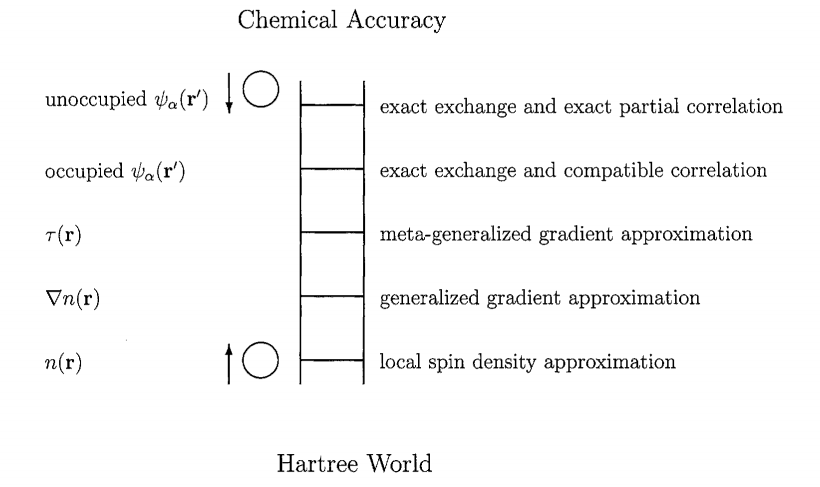
\includegraphics[width=12cm]{./gambar/tangga yakub.png}
    \caption{Skema \textit{Jacob's Ladders} yang dipopulerkan oleh \citeauthor{Perdew} yang menggambarkan tingkat akurasi fungsional dari terendah hingga tertinggi.}
    \label{fig:kpoints}
\end{figure}

Pendekatan LDA merupakan salah satu pendekatan awal dalam teori DFT, yang mempertimbangkan energi pertukaran-korelasi sebagai fungsi dari kepadatan elektron lokal pada setiap titik dalam ruang. LDA sederhana dan efisien dalam banyak kasus, tetapi sering kali tidak mampu menangkap efek kuantum yang lebih kompleks, seperti interaksi antara elektron yang lebih jauh. Sementara itu GGA merupakan perkembangan lebih lanjut dari LDA, di mana energi pertukaran-korelasi dinyatakan sebagai fungsi dari gradien kepadatan elektron. Pendekatan ini mempertimbangkan perubahan kepadatan elektron di seluruh sistem, memungkinkan pengambilan data spasial yang lebih baik dan hasil yang lebih akurat, terutama dalam kasus di mana interaksi antara elektron jarak jauh berperan signifikan.

Kedua kelas pendekatan ini, LDA dan GGA, memiliki kelebihan dan keterbatasan masing-masing dalam mengestimasi energi pertukaran-korelasi. Pemilihan pendekatan yang tepat tergantung pada sistem yang sedang diinvestigasi dan tingkat akurasi yang diinginkan dalam perhitungan kimia kuantum. Pada dasarnya, fungsional pertukaran-korelasi membantu mengkonversi distribusi kepadatan elektron ke dalam energi total sistem, memungkinkan simulasi komputasi yang akurat tentang sifat kimia, fisika, dan sifat material. Pengembangan fungsional pertukaran-korelasi yang lebih baik menjadi fokus dalam penelitian kimia kuantum, karena pengaruhnya terhadap keakuratan hasil perhitungan dalam berbagai konteks, mulai dari struktur molekul hingga reaksi kimia kompleks.
Dalam praktiknya, para ilmuwan sering menggunakan pendekatan dan aproksimasi yang berbeda dalam mengembangkan fungsional pertukaran-korelasi baru, karena tidak ada pendekatan yang sempurna untuk mengatasi kompleksitas interaksi elektron dalam sistem \textit{many-body}. Oleh karena itu, pemahaman tentang fungsional pertukaran-korelasi memiliki dampak signifikan dalam interpretasi hasil perhitungan teori densitas dan dalam pengembangan material dan senyawa baru dengan sifat-sifat unik.

%=====================================================================
\section{Quantum ESPRESSO}
%=====================================================================
\begin{figure}
    \centering
    
\includegraphics[width=10cm]{./gambar/qelogo.png}
    \caption{Logo Quantum ESPRESSO}
    \label{fig:kpoints}
\end{figure}
Quantum ESPRESSO adalah perangkat lunak simulasi fisika yang memungkinkan pengguna untuk melakukan perhitungan teoritis tentang sifat elektronik dan atomik material menggunakan metode mekanika kuantum. Perangkat lunak ini dikembangkan oleh sebuah tim internasional ahli dalam bidang fisika teoritis dan komputasi, dan dirilis sebagai proyek \textit{open source} yang tersedia secara gratis untuk digunakan oleh siapa saja. Tujuan utama dari Quantum ESPRESSO adalah untuk menyediakan alat yang dapat digunakan untuk memahami dan meramalkan sifat bahan secara lebih akurat dan efisien daripada metode eksperimental yang mahal dan rumit. Dalam upaya untuk mencapai tujuan ini, Quantum ESPRESSO menggunakan berbagai teknik mekanika kuantum, termasuk teori fungsional densitas (DFT), yang memungkinkan pengguna untuk memodelkan dan memprediksi sifat material seperti struktur kristal, energi ikatan, dan spektrum elektronik.

Quantum ESPRESSO dirancang untuk digunakan oleh para ilmuwan dan peneliti di berbagai bidang, termasuk fisika, kimia, dan teknik material. Perangkat lunak ini dapat digunakan untuk mempelajari berbagai jenis material, seperti logam, senyawa, dan material organik. Dalam pengembangan dan penggunaan Quantum ESPRESSO, para peneliti dapat menghasilkan pemahaman yang lebih baik tentang sifat material yang kompleks, memprediksi sifat material baru, dan mempercepat pengembangan teknologi baru. Quantum ESPRESSO memiliki beberapa fitur dan komponen penting yang memungkinkan pengguna untuk melakukan simulasi fisika dan analisis material. Salah satu fitur utama dari Quantum ESPRESSO adalah Modul PWSCF (\textit{Plane-Wave Self-Consistent Field}), yang menyediakan algoritma yang efisien untuk memecahkan persamaan \schro yang rumit dan memprediksi sifat elektronik material. Selain itu, Quantum ESPRESSO juga memiliki modul untuk memprediksi sifat getaran kristal, dinamika molekuler, dan sifat termodinamika material.

Dengan Quantum ESPRESSO, para ilmuwan dapat menghasilkan hasil simulasi dan analisis yang sangat berguna dan dapat dimanfaatkan dalam berbagai aplikasi. Misalnya, Quantum ESPRESSO dapat digunakan untuk merancang bahan baru dengan sifat khusus, seperti kekuatan yang lebih tinggi atau kemampuan konduktivitas listrik yang lebih baik. Selain itu, Quantum ESPRESSO dapat digunakan untuk mempelajari sifat material dalam kondisi yang ekstrem, seperti suhu dan tekanan yang sangat tinggi atau rendah. Secara keseluruhan, Quantum ESPRESSO adalah alat yang sangat berguna bagi para ilmuwan dan peneliti yang tertarik dalam memahami sifat material secara lebih mendalam dan meramalkan sifat material baru yang belum terungkap. Dengan penggunaan Quantum ESPRESSO, para ilmuwan dapat mempercepat pengembangan teknologi baru dan memberikan kontribusi yang signifikan dalam pemahaman kita tentang dunia material. 




\newpage
